\section{Graphs in Boolean world}
\label{sec:data_structure}

\begin{flushright}
  As an old Chinese philosopher never said, "Words about graphs are \\ worth a
  thousand pictures." \\ 
  -- \textbf{William Saffire}, \emph{The English Language} \\
  The New York Times, Sep 11, 2009
\end{flushright}

\paragraph{Lobbying for graphs}

  Data-structures such as array, list, vector, map, dictionary etc. are very
  useful. However, graphs has its own place among the titans.  Many
  algorithms become easier to visualize when we make use of graphs on paper;
  proofs are easy to state and understand. 

  Moreover, from the point of view of a programmer, coding with graph is
  convenient since sophisticated graph libraries are available in almost all
  self-respecting languages. Of course, there is a price to pay for this
  convenience : graphs consume relatively more memory to construct. Where
  available memory size is limited, such as on embedded systems, one may not be
  able to use graphs. One has to rewrite his algorithm which works on less costly
  data-structures.

  In 1975, there was only one book available on graph theory. It was written by
  Koing in German (\texttt{Theorie der Endlichen und Unendlichen Graphen}).
  (Later, William Tutte translated this book into English.) In
  its early years, graph theory was often looked upon with condescend by some
  mathematician. "The slum of topology" was the derisive remark they used to pass. 

  Since then graphs has emerged out of "the slum of topology" to become one of
  the most extensively studied mathematical structure.

  Narsingh Deo book "\textbf{Graph theory} with applications to engineering and
  computer science" is a very good introductory book on graph-theory for
  engineers. H. Narayan's "Submodular function and Electrical Network",
  especially chapter 3, gives an excellent overview of graphs in networks.
  
\paragraph{Libraries}

  There are many graph libraries available. No language which claims to be a
  contender for algorithmic design can exists without a graph library. We
  recommend using \textbf{Boost libraries} or \textbf{LEDA graph libraries} for
  C++. Boost graph libraries bindings are available for python, package
  \textbf{graph-tool}.  Python's native graph library \textbf{networkx} can also
  be used for small graph applications. Networkx has great many routines but it
  is not recommended for very large graphs for speed of networkx is not very
  good compared to graph-tool.

\paragraph{String graph to files}

   Format \textbf{dot} and \textbf{graphml} are two modern graph-formats. We'll
   use graphml to encode/decode our graph to a file. Both boost and LEDA
   libraries can read and write graphs to graphml format. This is a text-based
   format and can be read by humans.

\subsection{Graph as Boolean expression trees}

    In many of these project problems, we'll be working with Boolean expressions
    as input to the program or as intermediate data.  There are many ways to
    feed a Boolean expressions to a computer program. We need to fix a standard
    such that data can be transferred from one program to another without any
    hassle. 

    Boolean expressions can be encoded as expression-trees. What are expression
    trees? Mimicking Dodo the bird of 'Alice in Wonderland', one is temped to
    conclude that the best way to explain it is to show it. 

    On paper, Boolean expressions are written using standard symbols.  Table
    \ref{table:symbols} summarises them.

    \begin{figure}[h]
      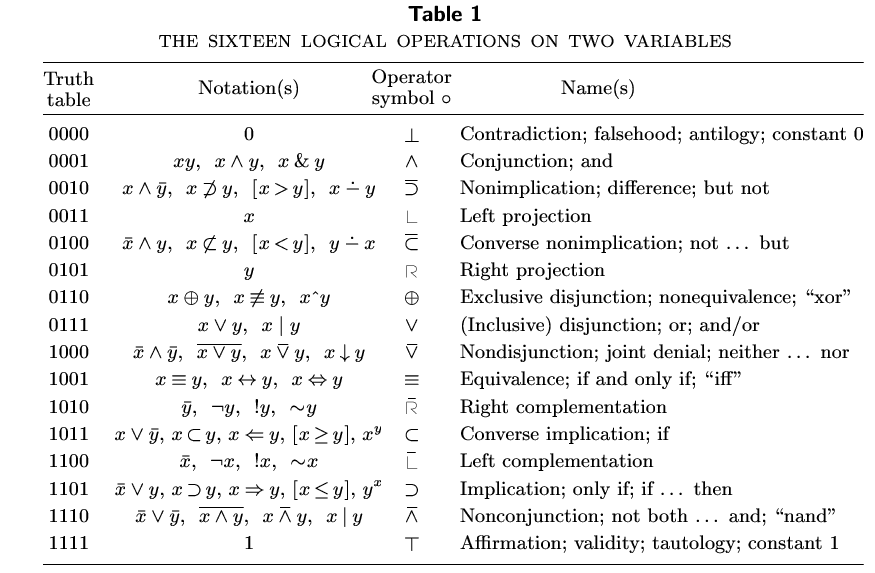
\includegraphics[width=\textwidth]{./figs/symbols.png}
      \caption{\small From Knuth, TAOP, 4A}
      \label{table:symbols}
    \end{figure}
    
    Consider the following expression. We are using standard Boolean symbols in these
    expressions.

    \begin{equation}
    \label{eq:expr1}
    y = (x_1 \vee x'_2) \wedge (x_2 \vee x_3) \wedge (x'_1 \vee x'_3)
    \end{equation}

    \begin{figure}[h]
    \centering
    \subfloat[]{
    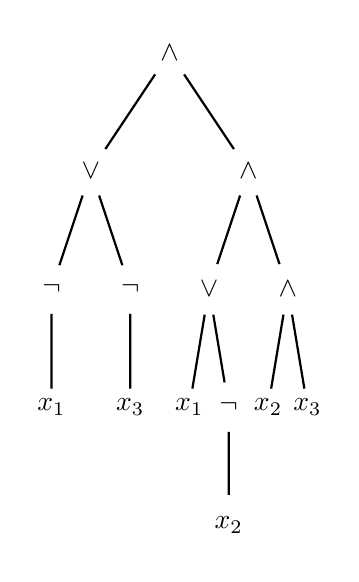
\begin{tikzpicture}
    [level distance = 15mm, thick,
      every node/.style={circle},
      level 1/.style={sibling distance=20mm,}, %
      level 2/.style={sibling distance=10mm,}, % nodes={fill=red!20}},
      level 3/.style={sibling distance=5mm,}, % nodes={fill=red!10}}
     ]
    \node {$\wedge$}
    child {node {$\vee$}
      child {node {$\neg$}
        child {node[rectangle] {$x_1$}}
       }
      child {node {$\neg$}
        child {node[rectangle] {$x_3$}}
       }
    }     
    child {node {$\wedge$}
      child {node {$\vee$}
        child {node[rectangle] {$x_1$}}
        child {node {$\neg$}
          child {node {$x_2$}}
         }
      }
      child {node {$\wedge$}
        child {node [rectangle] {$x_2$}}
        child {node [rectangle] {$x_3$}}
       }
     }
      ;
    \end{tikzpicture}
    }
    \subfloat[]{
    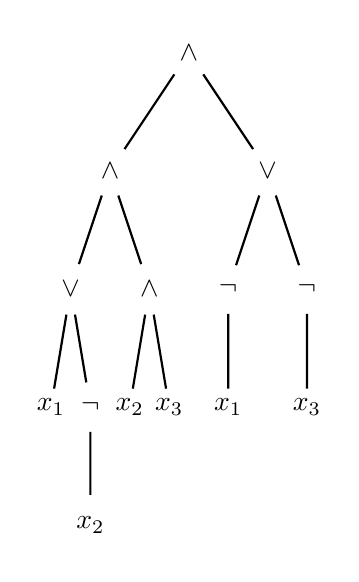
\begin{tikzpicture}
    [level distance = 15mm, thick,
      every node/.style={circle},
      level 1/.style={sibling distance=20mm,}, %
      level 2/.style={sibling distance=10mm,}, % nodes={fill=red!20}},
      level 3/.style={sibling distance=5mm,}, % nodes={fill=red!10}}
     ]
    \node {$\wedge$}
     child {node {$\wedge$}
      child {node {$\vee$}
        child {node[rectangle] {$x_1$}}
        child {node {$\neg$}
          child {node {$x_2$}}
         }
      }
      child {node {$\wedge$}
        child {node [rectangle] {$x_2$}}
        child {node [rectangle] {$x_3$}}
       }
     }
    child {node {$\vee$}
      child {node {$\neg$}
        child {node[rectangle] {$x_1$}}
       }
      child {node {$\neg$}
        child {node[rectangle] {$x_3$}}
       }
    }     
    ;
    \end{tikzpicture}
   }

   \caption{Two possible expression-trees of Boolean expression described in
     equation \ref{eq:expr1}. Some other representations are also possible.
     Since we have proved associativity in Boolean algebra, both of these trees
     are functionally equivalent. Although it is not at all easy to show that
     two given  expression trees are functionally equivalent or not.}
   \label{fig:expr_tree} 
 
 \end{figure}

    We'll use \texttt{not}, \texttt{and}, \texttt{or} to describe gates while
    writing these expressions. In special cases, such as technology mapping, one
    can also use additional \texttt{xor}, \texttt{nor}, and \texttt{nand} in
    output graph \footnote{A detailed standard should be made available on
      wiki}.  Figure \ref{fig:expr_tree} encodes these expression into an
    expression tree.
  

Three problems are immediate.
  
  \begin{problem}[15]
  \label{prob:expr_tree_to_minterms}
  Given a Boolean expression tree, construct another graph where each node
  represents a minterm of function. And an edge is drawn between two nodes whenever
  their Hamming distance is 1.
\end{problem}

  Such a graph could be an input to Quine McClusky algorithm which works over
  graphs (as we have discussed during project-session).

  \begin{problem}[25]
  \label{prob:minimize_expression_tree}
  Given a Boolean expression tree, minimize the Boolean function represented.
  \ref{prob:expr_tree_to_minterms}.   
  
  \end{problem}

  \begin{problem}[45]
  \label{prob:equivalence_checking}
  Given two Boolean expression trees, check if both expressions trees represents
  same Boolean function or not.
  \end{problem}


  \begin{remark}[HDL to Boolean expression-trees]

    Is there any way to construct Boolean expression tree out of a verilog
    design? Well, there seems to be one and TA of this course should give you a
    program to do this.

    Computer program \textbf{vis} can convert a verilog design to a
    \textbf{bliff} file. All we have to do is to convert this bliff file into
    boolean expression tree. 
  
  \end{remark}


\newpage
\subsection{Graphs as Binary Decision Diagrams}

\begin{flushright}

In popular usage, the term BDD almost always refers to Reduced Ordered Binary
Decision Diagram (ROBDD in the literature, used when the ordering and reduction
aspects need to be emphasized). The advantage of an ROBDD is that it is
canonical (unique) for a particular function and variable order. This
property makes it useful in functional equivalence checking and other operations
like functional technology mapping. \\
-- \textbf{Wikipedia}, The free encyclopedia (Accessed Sep 22, 2012) 

\end{flushright}

  One more way to encode a Boolean expression is BDD (Binary Decision
  Diagrams) which can been seen as recursive composition of
\textbf{If-then-else} logic.

  \paragraph{If-Then-Else}
  A Boolean function $f(x_1,\ldots,x_n)$ can be decomposed as following :
  \begin{equation}
    \begin{gathered}
      \begin{aligned}
        f(x_1,\ldots,x_n) &= {x'_1} \vee g(x_2,\ldots,x_n) \wedge {x_1} \vee
        h(x_2,\ldots,x_n), \text{where} \\
        g(x_2,\ldots,x_n) &= f(0,x_2,\ldots,x_n) \\
        h(x_2,\ldots,x_n) &= f(1,x_2, \ldots, x_n) \\
      \end{aligned}
    \end{gathered}
  \end{equation}

  This can be read as (ignoring function argument) : \textbf{if} $x_1=0$
  \textbf{then} $f = g$ \textbf{else} $f=h$. For electrical engineer, it is well
  known multiplexer. 


  \begin{figure}[h]
    \centering
    \subfloat[Mux]{
    \begin{tikzpicture}[circuit logic US]
      %% Dilawar Singh (c) 2012 
%% Circuit macros to produce amazing quality macros. More amazing and powerpuff
%% girls.
\def\mux { -- ++(0,-1) node [above right] {$1$} -- ++(0.6,0.2) -- 
++(0,0.6) -- ++(-0.6,0.2) -- cycle};
\def\muxr { -- node [below left] {$1$} ++(1,0) -- ++(-0.2,-0.6) -- 
++(-0.6,0) -- ++(-0.2,0.6)  -- cycle};

%% Multiplexor 
%% 3 params : location, size, name.
%% Note : To connect wires to north, east, south and west one should 
%% also use .center with name.
\newcommand{\multiplexer}[3]{
\draw #1 -- ++(0,-#2/4)  node (#3_input1) at ++(0,0) {\scriptsize{\hspace{8pt}1}}
-- ++(0,-#2/2) node (#3_input2) at ++(0,0){\scriptsize{\hspace{8pt}0}} 
-- ++(0,-#2/4) -- ++(#2/2,#2/4)
-- ++(0,#2/4) node(#3_output) [] {}  -- ++(0,#2/4) 
-- ++(-#2/4,#2/8) node(#3_select) {} -- ++(-#2/4,#2/8)
};

%% Register 
%% 4 parama : location, width, height, name 
%% Note : To connect wires to north, east, south and west one should 
%% also use .center with name.
\newcommand{\register}[4]{
\draw #1 -- ++(#2/2,0) node(#4_north){} --++(#2/2,0) 
% eastern side
-- ++(0,-#3/2) node(#4_east){} -- ++(0,-#3/2) 
% southern side 
-- ++(-#2/2,0) node(#4_south){} --++(-#2/2,0) 
% label 
-- ++(0,#3) node at ($#1+(#2/2+0.1,-#3/2)$) {#4} 
% the western triangle
-- ++(0.6*#3, -0.5*#3) -- ++(-0.6*#3, -0.5*#3)
% the western anchor
-- ++(0,#3/2) node (#4_west) {} 
};

%% Bus
%% 3 params : from, to, size 
\newcommand*{\bus}[4] {
\draw[->] #1 -- #2 node[midway]{\tiny{/}} 
    node [#3] {\scriptsize{#4}}
}

      \multiplexer{(2,0)}{2}{a};
      \node (h) at (1,-0.5) {$h$};
      \node (g) at (1,-1.5) {$g$};
      \draw[->] (h) -- (a_input1.center);
      \draw[->] (g) -- (a_input2.center);
      \draw[<-] (a_select.center) -- ++(0,0.5) node[above] {$x_1$};
      \draw[->] (a_output.center) -- ++(0.5,0) node[right] {$f$};
    \end{tikzpicture}
  }
  \subfloat[Graph of $f$]{
    \begin{tikzpicture}
      \node {$x_1$} 
        child[dotted] {node {$g$}}
        child {node {$h$}}
        ;
    \end{tikzpicture}
  }
  \caption{\textbf{If-Then-Else} operator. In (a) we have corrosponding
  circuit, which is a mux. In (b), we have graphical representation of
  $f$. Dotted line indicates that on this branch $x_1=0$.}
  \end{figure}

  Variable $x_1$ does not appear in $g$ and $h$. One application of
\textbf{if-then-else} breaks a function on $n$ variables into two functions of
$n-1$ variables. We can apply \textbf{if-then-else} operator recursively till
we are left with constant function $0$ and $1$. Lets consider the following
expression.

    \begin{equation}
    \label{eq:expr2}
    y = (x_1 \vee x'_2) \wedge (x_2 \vee x_3) 
    \end{equation}

   Now, we can construct a diagram which shows the process of recursively
   applying the \textbf{if-then-else}. This process is illustrated below.

   \begin{figure}[h]
     \centering
     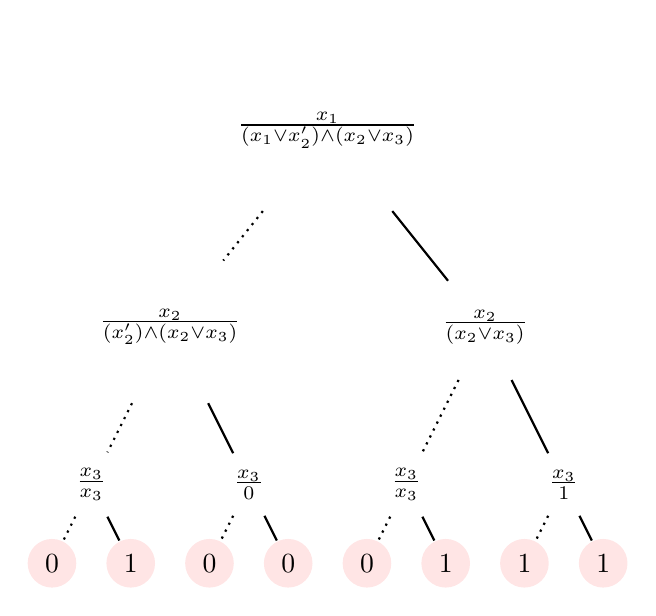
\begin{tikzpicture}
      [ 
        every node/.style={circle}, thick,
        level 1/.style={sibling distance=40mm, level distance=25mm,}, %
        level 2/.style={sibling distance=20mm, level distance=20mm,}, % nodes={fill=red!20}},
        level 3/.style={sibling distance=10mm, level distance=10mm
        ,nodes={fill=red!10}}
      ]
      \node {$\frac{x_1}{(x_1 \vee x'_2) \wedge (x_2 \vee x_3)}$}
        child[dotted] {node {$\frac{x_2}{(x'_2) \wedge (x_2 \vee x_3)}$}
          child[dotted] {node {$\frac{x_3}{ x_3}$}
            child[dotted] {node {$0$}}
            child[solid] {node {$1$}}
          }
          child[solid] {node {$\frac{x_3}{0}$}
            child[dotted] {node {$0$}}
            child[solid] {node {$0$}}
          }
        }
        child[] {node {$\frac{x_2}{(x_2 \vee x_3)}$}
          child[dotted] {node {$\frac{x_3}{x_3}$}
            child[dotted] {node {$0$}}
            child[solid] {node {$1$}}
          }
          child[] {node {$\frac{x_3}{1}$}
            child[dotted] {node {$1$}}
            child[solid] {node {$1$}}
          }
        }
       ;
     \end{tikzpicture}

     \caption{\small A graph diagram represents function described in equation
     \ref{eq:expr2}. A network of mux can be built form this graph. This kind of
   graph are called Binary Decision Diagrams. Usually reduced expression is not
   written below the variable name as we have written in this diagram.}
   
   \end{figure}

   A cursory look will reveal that this is very inefficient. We don't need so
   many nodes for $0$ and $1$. One node for each of them will suffice which can
   be shared by multiple edges by other nodes. Other simplifications are also
   possible which are discussed at length in your textbook.  Verify that
   following diagram also encode the same function but with fewer nodes. 

   \begin{figure}[h]
    \centering
    \begin{tikzpicture}
      [ node distance=5mm
        , every node/.style={}
      ]
      \node (x1) [, circle] {$x_1$};
      \node (x21) [circle, , below right=of x1] {$x_2$};
      \node (x20) [circle, , below left=of x1] {$x_2$};
      \draw[dotted] (x1) -- (x20);
      \draw[] (x1) -- (x21);
      \node (x30) [circle, , below left=of x20] {$x_3$};
      \node (x31) [circle, , below right=of x21] {$x_3$};
      \node (b0) [rectangle, draw , below right=of x30] {$0$};
      \node (b1) [rectangle, draw , below left=of x31] {$1$};

      \draw[dotted] (x20) -- (x30); 
      \draw (x20) to [bend left] (b0);
      \draw[] (x21) to [] (b1);
      \draw[dotted] (x21) to (x31);
      \draw[dotted] (x30) -- (b0);
      \draw (x30) to [bend left] (b1);

      \draw[dotted] (x31) to (b0);
      \draw[] (x31) to (b1);

    \end{tikzpicture}
    \caption{\small A \textbf{Reduced-Order BDD} of function described in equation
        \ref{eq:expr2}. Note that we have chosen $x_1$ first, followed by $x_2$
        and then $x_3$. Any other ordering will also produce a ROBDD. What is
        important that for a given ordering, generated ROBDD is unique. Size of ROBDD
        is know to be very sensitive to the ordering or variables.}
  \end{figure}

  \paragraph{BDD packages}

  Colarado university package \href{http://vlsi.colorado.edu/~fabio/CUDD/}{CUDD}
  maintained by Fabio Somenzi is widely used. Donald E. Knuth has also
  written a literate program for BDD which can be downloaded from his homepage. 

  \paragraph{Further reading}

  BDD's are discussed extensively in your textbook. You can also
  read \href{www.cs.cmu.edu/~bryant/pubdir/ieeetc86.pdf}{Byrant paper}. An
  elementry implemention of BDD was submitted last year. You can ask your TA for
  that code.

  \paragraph{BDD virtues}

  For a given ordering, ROBDD produced is unique. This is why they are
  theoretically attractive for representing Boolean expressions. Moreover, since
  two BDDs can be merged together efficiently on computer, they are very useful
  in solving many combinatorial problems.
   
  \begin{itemize}
    \item As we have seen that any BDD can be realised as a network of mux which
      can be implemented as 4-LUT on FPGA.
    \item The problem of satifiability of a Boolean expression is reduced to
    finding a path from root node to node \tikz \node[rectangle, draw] {$1$};.
    Not only we can prove whether a function is satisfiable or not, we can
    enumerate all combination of variable which satisfies the function.
    \item Add some more here.
  \end{itemize}

  \begin{problem}[20]
    
    Draw BDDs which are not satifiable i.e. there is
    no path between root node and node \tikz \node[draw, rectangle] {$1$};. If
    we can draw such BDDs using a program, we can definately convert it back to
    a Boolean expression which is not satisfiable.
  
  \end{problem}


  \begin{problem}[40]

    Given a expression tree, convert it to ROBDD for various variable ordering.
    Also generate all minterms from ROBDD.  Write down the variable ordering and
    reduced Boolean expression. Convince yourself that for different ordering,
    differnt expressions are generated?  Can you show that for the optimal
    ordering of the variables, size of Boolean expression generated from ROBDD
    is not worse that that of generated by Quine McClusky?
  
  \end{problem}

  \begin{comment}
    The classic problem of finding a minimum size Disjuntive Normal Form of a
    Boolean function can also be solved using ROBDD. Oliver Coudert has given
    an excellent overview in \textit{Integration} (1994), pp 97-140.
  \end{comment}


